
\chapter{Simplified Models for Locomotion\label{chapter:simplified_model_for_locomotion}}  %

\ifpdf
    \graphicspath{{chapter_simplified_models/figures/Raster/}{chapter_simplified_models/figures/PDF/}{chapter_simplified_models/figures/}}
\else
    \graphicspath{{chapter_simplified_models/figures/Vector/}{chapter_simplified_models/figures/}}
\fi

In Chapter~\ref{chapter:floating_base_system_modeling} we present the kinematics and the dynamics of a floating base system. In this chapter, we present some approximations of the centroidal dynamics presented in Section~\ref{sec:centroidal-dynamics} by assuming some simplifying hypotheses. The tools introduced in this chapter will be considered in the design of the simplified model controllers presented in Chapter~\ref{chapter:simplified_benchmarking}.
\par
Assuming that a robot makes a single contact with the environment while keeping a constant center of mass height, the robot's centroidal dynamics can be approximated to the well-known Linear Inverted Pendulum (LIPM)~\citep{Kajita2001, Kajita2003} and the Capture Point model~\citep{Pratt2006}. These two models assume constant angular momentum and approximate the center of mass dynamics with a linear time-invariant dynamical system, making the study of a feasible trajectory for the center of mass simpler. The LIPM and the CP became very popular along with the Zero Moment Point (ZMP) as a contact feasibility criterion~\citep{Vukobratovic1969}. Similar to the ZMP, the centroidal moment pivot (CMP) has a widespread diffusion in the modeling and control of floating base system~\citep{Li2020Centroidal-momentum-basedLocomotion,Seyde2018InclusionWalking,Hopkins2015,Popovic2005,Shafiee-Ashtiani2017PushControl}. The definition of the CMP is pivotal in considering a variable centroidal angular momentum while generating a feasible CoM trajectory. Indeed, when the CMP corresponds to the ZMP the centroidal angular momentum remains constant. 
\cite{Englsberger2011,Englsberger2015} extends the Capture Point in the 3D scenario, defining the \emph{Divergent Component of Motion} (DCM). The DCM is a linear combination of the center of mass position and velocity. By definition, the CoM can be indirectly
stabilized by tracking an appropriate DCM trajectory. The DCM model assumes a constant natural frequency of the LIPM for trajectory planning. As a consequence, the ZMP can deviate from the desired reference when the vertical CoM dynamics does not match the time-invariant LIPM dynamics.
\cite{Hopkins2015} attempt at loosening this assumption by extending the DCM to consider a time-varying natural frequency.
\par
In this chapter, we present a short overview of the simplified models that are often exploited by the robot locomotion community. In particular, Section~\ref{sec:lip} introduces the LIPM. Section~\ref{sec:zmp} and \ref{sec:cmp} present the ZMP and CMP, respectively. We introduce the DCM in Section~\ref{sec:dcm}. Finally, Section~\ref{sec:dcm-tv} extends the definition of DCM to the time-varying case. 



  
\tikzset {_rh5m64a0t/.code = {\pgfsetadditionalshadetransform{ \pgftransformshift{\pgfpoint{89.1 bp } { -108.9 bp }  }  \pgftransformscale{1.32 }  }}}
\pgfdeclareradialshading{_ify870utn}{\pgfpoint{-72bp}{88bp}}{rgb(0bp)=(1,1,1);
rgb(0bp)=(1,1,1);
rgb(25bp)=(0,0,0);
rgb(400bp)=(0,0,0)}
\tikzset{every picture/.style={line width=0.75pt}} %

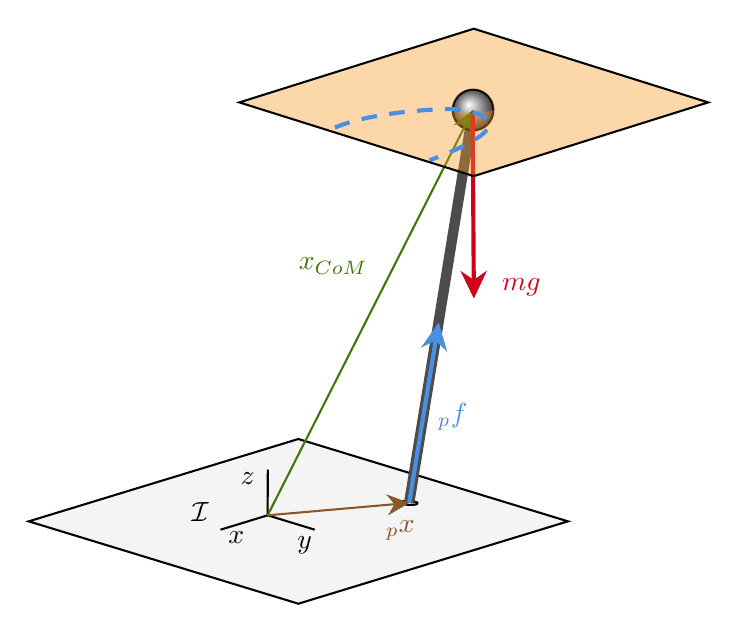
\begin{tikzpicture}[x=0.75pt,y=0.75pt,yscale=-1,xscale=1]

\draw  [fill={rgb, 255:red, 244; green, 244; blue, 244 }  ,fill opacity=1 ] (225.09,285.85) -- (355,325.53) -- (225.09,365.21) -- (95.17,325.53) -- cycle ;
\draw    (210.36,300.63) -- (210.29,322.62) ;
\draw    (187.59,329.55) -- (210.29,322.62) ;
\draw    (232.99,329.55) -- (210.29,322.62) ;
\draw  [fill={rgb, 255:red, 255; green, 255; blue, 255 }  ,fill opacity=1 ] (276.63,317.42) .. controls (274.56,317.1) and (273.7,316.49) .. (274.71,316.07) .. controls (275.73,315.64) and (278.23,315.56) .. (280.3,315.88) .. controls (282.38,316.2) and (283.24,316.81) .. (282.22,317.23) .. controls (281.21,317.66) and (278.71,317.74) .. (276.63,317.42) -- cycle ;
\draw [color={rgb, 255:red, 76; green, 76; blue, 76 }  ,draw opacity=1 ][line width=3.75]    (309.06,128.71) -- (278.47,316.65) ;
\draw [color={rgb, 255:red, 74; green, 144; blue, 226 }  ,draw opacity=1 ][fill={rgb, 255:red, 74; green, 144; blue, 226 }  ,fill opacity=1 ][line width=1.5]    (278.47,316.65) -- (292.02,233.62) ;
\draw [shift={(292.67,229.67)}, rotate = 99.27] [fill={rgb, 255:red, 74; green, 144; blue, 226 }  ,fill opacity=1 ][line width=0.08]  [draw opacity=0] (13.4,-6.43) -- (0,0) -- (13.4,6.44) -- (8.9,0) -- cycle    ;
\draw [color={rgb, 255:red, 139; green, 87; blue, 42 }  ,draw opacity=1 ]   (210.29,322.62) -- (275.48,316.91) ;
\draw [shift={(278.47,316.65)}, rotate = 175] [fill={rgb, 255:red, 139; green, 87; blue, 42 }  ,fill opacity=1 ][line width=0.08]  [draw opacity=0] (10.72,-5.15) -- (0,0) -- (10.72,5.15) -- (7.12,0) -- cycle    ;
\path  [shading=_ify870utn,_rh5m64a0t] (299.45,127.33) .. controls (299.45,121.91) and (303.84,117.51) .. (309.27,117.51) .. controls (314.69,117.51) and (319.09,121.91) .. (319.09,127.33) .. controls (319.09,132.76) and (314.69,137.15) .. (309.27,137.15) .. controls (303.84,137.15) and (299.45,132.76) .. (299.45,127.33) -- cycle ; %
 \draw   (299.45,127.33) .. controls (299.45,121.91) and (303.84,117.51) .. (309.27,117.51) .. controls (314.69,117.51) and (319.09,121.91) .. (319.09,127.33) .. controls (319.09,132.76) and (314.69,137.15) .. (309.27,137.15) .. controls (303.84,137.15) and (299.45,132.76) .. (299.45,127.33) -- cycle ; %

\draw [color={rgb, 255:red, 65; green, 117; blue, 5 }  ,draw opacity=1 ]   (210.29,322.62) -- (307.91,130.01) ;
\draw [shift={(309.27,127.33)}, rotate = 116.88] [fill={rgb, 255:red, 65; green, 117; blue, 5 }  ,fill opacity=1 ][line width=0.08]  [draw opacity=0] (10.72,-5.15) -- (0,0) -- (10.72,5.15) -- (7.12,0) -- cycle    ;
\draw [color={rgb, 255:red, 208; green, 2; blue, 27 }  ,draw opacity=1 ][line width=1.5]    (309.06,128.71) -- (309.61,214.12) ;
\draw [shift={(309.64,218.12)}, rotate = 269.63] [fill={rgb, 255:red, 208; green, 2; blue, 27 }  ,fill opacity=1 ][line width=0.08]  [draw opacity=0] (13.4,-6.43) -- (0,0) -- (13.4,6.44) -- (8.9,0) -- cycle    ;
\draw  [draw opacity=0][fill={rgb, 255:red, 245; green, 152; blue, 35 }  ,fill opacity=0.39 ] (422.54,123.69) -- (309.6,159.2) -- (196.66,123.69) -- (309.6,88.18) -- (422.54,123.69) -- cycle (299.45,126.92) .. controls (302.28,127.97) and (305.55,128.61) .. (309.06,128.71) .. controls (312.71,128.81) and (316.14,128.3) .. (319.09,127.33) .. controls (319.09,127.23) and (319.1,127.13) .. (319.1,127.03) .. controls (319.1,121.61) and (314.7,117.21) .. (309.27,117.21) .. controls (303.89,117.21) and (299.51,121.55) .. (299.45,126.92) -- cycle ;
\draw [color={rgb, 255:red, 74; green, 144; blue, 226 }  ,draw opacity=1 ][line width=1.5]  [dash pattern={on 5.63pt off 4.5pt}]  (242.71,135.81) .. controls (262.06,127.58) and (296.15,126.71) .. (299.45,126.92) .. controls (302.75,127.12) and (343.67,130.76) .. (288.35,151.56) ;
\draw   (309.6,88.18) -- (422.54,123.69) -- (309.6,159.2) -- (196.66,123.69) -- cycle ;

\draw (321.7,207.22) node [anchor=north west][inner sep=0.75pt]    {$\textcolor[rgb]{0.82,0.01,0.11}{mg}$};
\draw (195.77,300.38) node [anchor=north west][inner sep=0.75pt]    {$z$};
\draw (189.83,328.97) node [anchor=north west][inner sep=0.75pt]    {$x$};
\draw (223.06,331.58) node [anchor=north west][inner sep=0.75pt]    {$y$};
\draw (172.19,314.83) node [anchor=north west][inner sep=0.75pt]    {$\mathcal{I}$};
\draw (223.79,197.17) node [anchor=north west][inner sep=0.75pt]    {$\textcolor[rgb]{0.25,0.46,0.02}{x}\textcolor[rgb]{0.25,0.46,0.02}{_{\text{CoM}}}$};
\draw (265.89,323.65) node [anchor=north west][inner sep=0.75pt]    {$\textcolor[rgb]{0.55,0.34,0.16}{_{\text{p}}}\textcolor[rgb]{0.55,0.34,0.16}{x}$};
\draw (290.85,267.22) node [anchor=north west][inner sep=0.75pt]    {$\textcolor[rgb]{0.29,0.56,0.89}{_{\text{p}}}\textcolor[rgb]{0.29,0.56,0.89}{f}$};


\end{tikzpicture}


\section{The zero moment point}\label{sec:zmp}
Consider a rigid body that makes a contact with a surface and assume that:
\begin{enumerate}
    \item there exists an inertial frame $\mathcal{I}$;
    \item there exist a frame $B$ rigidly attached to the body and we denote $o_B$ the origin of the frame and $[B]$ its orientation;
    \item there exists a contact domain $\Omega \in \mathbb{R}^3$, we denote with ${}^B x$ a point in the contact surface expressed in the the frame $B$;
    \item $\forall \; {}^B x \in \Omega$ there exists a continuous pure force distribution that depends on the point location, i.e.,
    \begin{equation}
        \rho : \mathbb{R}^3 \longrightarrow \mathbb{R}^3.
    \end{equation}
\end{enumerate}
Given the above assumption, the contact torque distribution about a point $p_B$, $\sigma_{o_B} :  \mathbb{R}^3 \longrightarrow \mathbb{R}^3$ writes
\begin{equation}
    \sigma_{o_B} = {}^B x \times \rho({}^B x).
\end{equation}
Once the pure force and torque distribution are defined, then the equivalent left trivialized contact 6D force, i.e., in body frame writes as~\citep{Caron2015StabilityAreas}
\begin{equation}
    {}_B \mathrm{f} = \begin{bmatrix}
    {}_B f \\
    {}_B \mu
    \end{bmatrix} = 
    \begin{bmatrix}
    \int_\Omega \rho \diff \Omega \\
    \int_\Omega \sigma_{o_B} \diff \Omega
    \end{bmatrix}.
\end{equation}
Let us introduce another frame $F[B]:= (o_F, [B])$ placed in the contact domain $\Omega$ as a frame that has its origin in $o_F$ and is oriented as $B$.
Now we aim to find the origin $o_F$ such that the tangential component of the angular term of ${}_{F[B]} \mathrm{f}$ is equal to zero, i.e., $e_4^\top {}_{F[B]} \mathrm{f} = e_5^\top {}_{F[B]} \mathrm{f} = 0$.
The location of the origin $o_F$ is crucial in the study of the contact dynamic balance, which is achieved by ensuring that the contact area $\Omega$ remains invariant. If $o_F$ exists and belongs to the contact domain, i.e., $o_F \in \Omega$ the contact dynamic balance is ensured and $o_F$ is equivalent to the Zero Moment Point (ZMP), often denoted by $x_\text{ZMP}$. Otherwise, if $o_F \notin \Omega$, then $x_\text{ZMP}$ is not defined and the rigid body will rotate.  
This statement is generally denoted by the ZMP condition~\citep{Arakawa1997NaturalLayers},  also known as the ZMP stability criterion~\citep{Li1998LearningTrunk}.
\par
Given a 6D force ${}_B \mathrm{f}$, if the ZMP exists, it is given by~\citep{vukobratovic2004zero}:
\begin{equation}
    \label{eq:zmp_definition}
    {}^B x_\text{ZMP} = \begin{bmatrix}
    - \frac{{}_B\mu_y}{{}_Bf_z} \\
    \frac{{}_B\mu_x}{{}_Bf_z}
    \end{bmatrix}.
\end{equation}
The concept of ZMP has been frequently used in robot control~\citep{Hirai1998TheRobot,Shih1996TheFreedom,Kajita2003,Kajita2010BipedTracking} as a criterion of postural stability, however, we observe that:
\begin{enumerate}
    \item the term \emph{zero} moment point is misleading since, in general, only two of the three moments components are zero; 
    \item even if the ZMP criterion is satisfied, the contact may not be \emph{weak contact stable}~\footnote{A contact is weakly stable if an only if~\citep{Caron2015StabilityAreas}: i)the relative velocity and acceleration of the contact are zero, ii) the 6D wrench belongs to the wrench cone.}. In fact, the ZMP can be defined, but the pure force ${}_{F[B]}\mathrm{f}$ may not belong to the friction cone. 
\end{enumerate}
Despite these weaknesses of the ZMP condition, the criterion is widely used with the LIPM where weakly stability of the contact is considered as a hypothesis. Combining the definition of the ZMP with the LIP the CoM dynamics becomes
\begin{equation}\label{eq:lip_zmp_dynamics}
	\ddot{x}_\text{LIP} = \zeta^2\left(x_\text{LIP} - {}^\mathcal{I} H _ B \; {}^B x_{\text{ZMP}}\right).
\end{equation} 
\subsection{Connection between the ZMP and the centroidal momentum dynamics}
Given a multi-body system that makes a contact with the environment. Consider a rigidly attached frame to the contact surface $B:=(o_B, [B])$ and a frame placed on the CoM, $G[B]:=(x_\text{CoM}, [B])$, that has its origin in the center of mass $x_\text{CoM}$ and is oriented as $B$. The centroidal dynamics of the system~\eqref{eq:centroidal_momentum_dynamics} is given by
\begin{equation}
\label{eq:zmp_centroidal}
    {}_{G[B]} \dot{h} =  \begin{bmatrix}
     {}_{G[B]} \dot{h}^p \\
      {}_{G[B]} \dot{h}^\omega
    \end{bmatrix} = {}_{G[B]} X ^ B {}_B \mathrm{f} + m \bar{g}.
\end{equation}
Substituting ${}_B\mathrm{f}$ from~\eqref{eq:zmp_centroidal} into~\eqref{eq:zmp_definition}, we write a relationship between the ZMP and the centroidal momentum as
\begin{equation}
    \label{eq:zmp_centroidal_relationship}
    {}^B x_\text{ZMP} = \begin{bmatrix}
    {}^B x_{\text{CoM}_x} - \frac{ {}_{G[B]} \dot{h}^\omega_y}{ {}_{G[B]} \dot{h}^p_z + m \| \bar{g} \|} - {}^B  x_{\text{CoM}_z} \frac{ {}_{G[B]} \dot{h}^p_x}{{}_{G[B]} \dot{h}^p_z + m \| \bar{g} \|} \\
    {}^B  x_{\text{CoM}_y} + \frac{ {}_{G[B]} \dot{h}^\omega_x}{ {}_{G[B]} \dot{h}^p_z + m \| \bar{g} \|} - {}^B  x_{\text{CoM}_z} \frac{ {}_{G[B]} \dot{h}_y^p}{{}_{G[B]} \dot{h}_z^p + m \| \bar{g} \|}
    \end{bmatrix}.
\end{equation}
\begin{figure}[t]
\centering
    \begin{subfigure}[b]{0.48\textwidth}
        \centering
        \includegraphics{chapter_simplified_models/figures/zmp-cmp-different.tikz}
        \caption{}
        \label{fig:zmp-cmp-different}
    \end{subfigure}
    \hfill
    \begin{subfigure}[b]{0.48\textwidth}
        \centering
        \includegraphics{chapter_simplified_models/figures/zmp-cmp-equal.tikz}
        \caption{}
        \label{fig:zmp-cmp-equal}
    \end{subfigure}
	\caption[Relation between CMP and ZMP.]{The CMP is the point at which the ground reaction force must act to maintain the horizontal component of the centroidal angular momentum constant. The CMP corresponds with the ZMP when the rate of change of the centroidal angular momentum is zero - \ref{fig:zmp-cmp-equal}. When the centroidal angular momentum is not constant, the CMP and the ZMP are two different points.}
	\label{fig:cmp-zmp}
\end{figure}

\section{The centroidal moment pivot\label{sec:cmp}}
Given a multi-body system that interacts with its surroundings. Consider a frame that is rigidly coupled to the contact surface $B:=(o_B, [B])$ and a frame that is positioned on the CoM. The origin of $G[B]:=(x_\text{CoM}, [B])$ is at the center of mass $x_\text{CoM}$, and is oriented as $B$. The Centroidal Moment Pivot (CMP)~\citep{Popovic2005} is defined as the point where a line parallel to the contact force, passing through the CoM, intersects the contact surface. More formally, we define the CMP, denoted as $x_\text{CMP}$, as
\begin{equation}
\label{eq:cmp_definition}
    x_\text{CMP} \in \mathbb{R}^3\quad \text{such that } ({}^B x_\text{CMP} - {}^B x_\text{CoM}) \times {}_B f = 0, \; e_3 ^ \top {}^B x_\text{CMP} = 0.
\end{equation}
Expanding Equation~\eqref{eq:cmp_definition}, the components ${}^B x_\text{CMP}$ write as
\begin{IEEEeqnarray}{RCL}
	\IEEEyesnumber \phantomsection \label{eq:cmp_definition_explicit}
	{}^B x_{\text{CMP}_x} &=& {}^B x_{\text{CoM}_x} - \frac{{}_B f_x}{{}_B f_z} x_{\text{CoM}_z} , \IEEEyessubnumber\\
	{}^B  x_{\text{CMP}_y} &=& {}^B x_{\text{CoM}_y} - \frac{{}_B f_y}{{}_B f_z} x_{\text{CoM}_z}, \IEEEyessubnumber \\
	{}^B  x_{\text{CMP}_z} &=& 0. \IEEEyessubnumber
\end{IEEEeqnarray}
Combining Equation~\eqref{eq:zmp_centroidal_relationship} with the CMP definition~\eqref{eq:cmp_definition_explicit} we can express the CMP in terms of ZMP location, rate of change of the centroidal angular momentum, and the ground reaction force as
\begin{IEEEeqnarray}{RCL}
	\IEEEyesnumber \phantomsection \label{eq:cmp_definition_explicit_zmp}
	{}^B x_{\text{CMP}_x} &=& {}^B x_{\text{ZMP}_x} + \frac{{}_{G[B]} \dot{h}^\omega_y}{{}_B f_z} , \IEEEyessubnumber\\
	{}^B  x_{\text{CMP}_y} &=& {}^B x_{\text{ZMP}_y} - \frac{{}_{G[B]} \dot{h}^\omega_x}{{}_B f_z}, \IEEEyessubnumber \\
	{}^B  x_{\text{CMP}_z} &=& 0. \IEEEyessubnumber
\end{IEEEeqnarray}
To give the reader a better comprehension, we can image the CMP as the point where the ground reaction
force would have to act to keep the horizontal component of the whole-body angular momentum constant. When the centroidal angular momentum is constant, i.e., ${}_{G[B]} \dot{h}^\omega = 0_{3\times 1}$ the CMP coincides with the ZMP -- Figure~\ref{fig:cmp-zmp}. Moreover, while by definition the ZMP cannot leave the contact domain $\Omega$, the CMP, in the case of ${}_{G[B]} \dot{h}^\omega_x \neq 0$  or ${}_{G[B]} \dot{h}^\omega_y \neq 0$, can.
Let us assume that the motion of the multi-body system is approximated by the LIPM, i.e., the hypothesis in Section~\ref{sec:lip} holds, then it is possible to prove that the position of the CMP coincides with the ZMP.
To prove this statement, it is worth noticing that when the hypotheses of the LIPM are satisfied the centroidal angular momentum is kept constant -- Section~\ref{sec:lip}, hence, substituting ${}_{G[B]} \dot{h}^\omega$ into Equation~\eqref{eq:cmp_definition_explicit_zmp}, we can conclude that if the system is approximated by the LIPM, then the CMP and ZMP coincide.

\section{The divergent component of motion}\label{sec:dcm}
Given a multi-body system making $n_c$ contacts with the environment and having a mass equal to $m$. Let us consider an inertial frame $\mathcal{I}:=(o_\mathcal{I}, [\mathcal{I}])$. Let $\bar{G};=(x_\text{CoM}, [\mathcal{I}])$ a frame whose origin is located on the CoM of the multi-body system, while the orientation is parallel to the inertial frame $\mathcal{I}$. The CoM acceleration is given by:
\begin{equation}
    \label{eq:com_dynamics_dcm}
    \ddot{x}_\text{CoM} =  m g + {}_{\bar{G}} f,
\end{equation}
where ${}_{\bar{G}} f$ is the sum of all the external forces acting on the robot CoM.
The divergent component of motion (DCM)~\citep{Englsberger2011, Englsberger2013, Englsberger2015}, often denoted with $\xi$, is a linear transformation of the Center of Mass state:
\begin{equation}
  \label{eq:3d_dcm}
  \xi = x_\text{CoM} + b \dot{x}_\text{CoM},
\end{equation}
where $b \in \mathbb{R}_+$ is a strictly positive constant.

By reordering Equation \eqref{eq:3d_dcm} the CoM dynamics can be derived as
\begin{equation}
  \label{eq:com_3d_dcm}
  \dot{x}_\text{CoM} = -\frac{1}{b} (x_\text{CoM} - \xi).
\end{equation}
The CoM position is governed by a stable first-order system. 
It is worth noticing that given a desired DCM set-point $\xi(t) = \bar{\xi}$, the CoM position will converge to it, Indeed let us define the error $e$ as $e = x_\text{CoM} - \xi$, the error dynamics is $\dot{e} = - e / b$ which is an asymptotically stable system. 
\par
By differentiating \eqref{eq:com_3d_dcm} and combining it with \eqref{eq:3d_dcm} and \eqref{eq:com_dynamics_dcm}, the DCM dynamics holds:
\begin{IEEEeqnarray}{LL}
\IEEEyesnumber \phantomsection \label{eq:3d_dcm_dynamics_F}
    \dot{\xi} &= -\frac{1}{b}(x_\text{CoM} - \xi) + b \ddot{x}_\text{CoM} \IEEEyessubnumber\\
    &= -\frac{1}{b}(x_\text{CoM} - \xi) + \frac{b}{m} ( {}_{\bar{G}} f + m g)\IEEEyessubnumber.
  \end{IEEEeqnarray}

The main idea is to design the external forces to be appropriate for the robot's walking task while the feasibility constraints are satisfied (i.e., the center of pressure inside the support polygon).
For the sake of simplicity, a force-to-point transformation is used to express the external
forces:
\begin{equation}
    \label{eq:3d_dcm_external_force}
    {}_{\bar{G}} f = \gamma (x_\text{CoM} - x_\text{eCMP}),
\end{equation}
where $\gamma$ is a positive constant and eCMP is the enhanced centroidal moment pivot point
\citep{Englsberger2013, Englsberger2015}. It is important to point out that the eCMP
is related to the CMP \citep{Popovic2005}. The first one could not belong to the ground plane.
The second is the intersection point between the ground surface and the line between the CoM
and the eCMP.
Combining Equation \eqref{eq:3d_dcm_dynamics_F} with \eqref{eq:3d_dcm_external_force}, we rewrite the DCM as:
\begin{equation}
    \label{eq:3d_dcm_dynamics_com}
\dot{\xi} = \left(\frac{b\gamma}{m} - \frac{1}{b}\right)x_\text{CoM} + \frac{1}{b} \xi - \frac{b\gamma}{m} x_\text{eCMP} +  b g,
\end{equation}
this shows that the states $x_\text{CoM}$ and $\xi$ are in general coupled, however choosing the parameter $\gamma$ equal to $m/b^2$ the DCM dynamics~\eqref{eq:3d_dcm_dynamics_com} becomes independent of the CoM position
\begin{equation}
  \label{eq:3d_dcm_dynamics_eCMP}
  \dot{\xi} = \frac{1}{b} \xi - \frac{1}{b} x_\text{eCMP} +  b g.
\end{equation}
Let us introduce the virtual repellent point (VPR) as 
\begin{equation}
\label{eq:vrp}
x_\text{VRP} = x_\text{eCMP} + b^2 g,
\end{equation}
the DCM dynamics can be simplified as:
\begin{equation}
  \label{eq:3d_dcm_dynamics_vrp}
  \dot{\xi} = \frac{1}{b} (\xi - x_\text{VRP}).
\end{equation}
This shows that the 3D-DCM dynamic equation is a first-order unstable dynamic system $\forall b > 0$.
\par
Combining Equation~\eqref{eq:cmp_definition_explicit} with \eqref{eq:3d_dcm_external_force}, we can express the CMP in terms of the eCMP and the ground reaction force as:
\begin{IEEEeqnarray}{RCL}
	\IEEEyesnumber \phantomsection \label{eq:cmp_definition_explicit_ecmp}
	{}^B x_{\text{CMP}_x} &=& {}^B x_{\text{eCMP}_x} + \frac{b^2}{m} {}_{G[B]} f_x - \frac{{}_{G[B]} f_x}{{}_{G[B]} f_z} \left( x_{\text{eCMP}_z} + \frac{b^2}{m} {}_{G[B]} f_z \right) , \IEEEyessubnumber\\
	{}^B x_{\text{CMP}_y} &=& {}^B x_{\text{eCMP}_y} + \frac{b^2}{m} {}_{G[B]} f_y - \frac{{}_{G[B]} f_y}{{}_{G[B]} f_z} \left( x_{\text{eCMP}_z} + \frac{b^2}{m} {}_{G[B]} f_z \right) , \IEEEyessubnumber\\
	{}^B  x_{\text{CMP}_z} &=& 0. \IEEEyessubnumber
\end{IEEEeqnarray}

Finally, it is worth to notice that while moving the z coordinate of the eCMP will change, indeed combining~\eqref{eq:cmp_definition_explicit} with the CoM dynamics~\eqref{eq:com_dynamics_dcm} and projecting it on the z coordinate we obtain:
\begin{equation}
    \label{eq:ecmpz-comz}
    x_{\text{eCMP}_z} = x_{\text{CoM}_z} - b^2 \left(\ddot{x}_{\text{CoM}_z} + |g| \right).
\end{equation}
In other words, if the height of the CoM varies, the height of the eCMP will change accordingly. 
\subsection{Connection between the DCM and the LIPM \label{sec:2D-DCM}}
Let us assume that the motion of the multi-body system is approximated by the LIPM, i.e., the hypothesis in Section~\ref{sec:lip} holds, and $b$ is equal to the inverse of the LIPM time constant, that is, $b = 1/\zeta$, then it is possible to prove that:
\begin{enumerate}
    \item the position of the eCMP coincides with the CMP and the ZMP;
    \item the $z$ coordinate of the VRP and the DCM coincides with the CoM height.
\end{enumerate}
To prove the first statement, it is worth noticing that we should prove that the eCMP and the CMP coincide, indeed in Section~\ref{sec:cmp}, we already show that when the model is approximated by the LIPM the CMP and ZMP coincide. In the LIPM regime, the z component of the CoM acceleration is forced to be zero. So subsisting the assumption in \eqref{eq:ecmpz-comz} and making explicit $b$ we obtain:
\begin{equation}
    \label{eq:ecmpz-comz-lipm}
    x_{\text{eCMP}_z} = x_{\text{CoM}_z} - \frac{|g|}{\zeta} =  x_{\text{CoM}_z} - \frac{|g|}{|g|} x_{\text{CoM}_z} = 0.
\end{equation}
Now, substituting \eqref{eq:ecmpz-comz-lipm} into \eqref{eq:cmp_definition_explicit_ecmp}, we obtain that ${}^B x_{\text{CMP}} = {}^B x_{\text{eCMP}}$.
\par
To prove the second statement we can consider the CoM dynamics~\eqref{eq:com_3d_dcm} projected on the $z$ coordinate, since $\dot{x}_{\text{CoM}_z} = 0$, it becomes evident that $\xi_z = x_{\text{CoM}_z} = h$. By projecting \eqref{eq:3d_dcm_dynamics_vrp} on the $z$ coordinate, we have $\dot{\xi}_z = \frac{1}{b}(\xi_z - x_{\text{VRP}_z}) = 0$, hence $\xi_z = x_{\text{VRP}_z}$.
\par
Since the DCM dynamics is different from zero only in the planar coordinates, we define
\begin{equation}
	\xi_\text{LIP} = \begin{bmatrix}
	e_1^\top \\
	e_2^\top
	\end{bmatrix}\xi, \quad \xi_\text{LIP} \in \mathbb{R}^2,
\end{equation}
We then obtain the CoM and DCM dynamics if the LIP hypotheses are satisfied:
\begin{IEEEeqnarray}{LL}
\phantomsection \label{eq:dcm_dynamics_lipm}  \IEEEyesnumber  \IEEEyessubnumber*
    \dot{x}_\text{LIP} &= -\zeta\left(x_\text{LIP} - \xi_\text{LIP}\right), \label{eq:dcm_dynamics_lipm_com} \\
    \dot{\xi}_\text{LIP} &= \zeta\left(\xi_\text{LIP} - x_\text{ZMP}\right) \label{eq:dcm_dynamics_lipm_dcm}.
\end{IEEEeqnarray}

\section{The time-varying DCM\label{sec:dcm-tv}}
Given a multi-body system making $n_c$ contacts with the environment and having a mass equal to $m$, an inertial frame $\mathcal{I}:=(o_\mathcal{I}, [\mathcal{I}])$ and $\bar{G}:=(x_\text{CoM}, [\mathcal{I}])$. We previously show that the DCM dynamics is defined by~\eqref{eq:3d_dcm}, where the parameter $b$ is a constant positive number. The time-varying DCM~\citep{Hopkins2015} extends the DCM definition~\citep{Englsberger2015} to account for a natural frequency that changes over time. \cite{Hopkins2015} define the time-varying DCM as
\begin{equation}
    \label{eq:3d_dcm_tv}
    \xi = x_\text{CoM} + \eta(t) \dot{x}_\text{CoM}.
\end{equation}
where $\eta(t)$ is a strictly positive function such that $\eta(t)>\bar{\eta} > 0$
By reordering Equation \eqref{eq:3d_dcm_tv} the CoM dynamics can be derived as
\begin{equation}
  \label{eq:com_3d_dcm_tv}
  \dot{x}_\text{CoM} = -\frac{1}{\eta(t)} (x_\text{CoM} - \xi).
\end{equation}
The CoM position is governed by an asymptotically stable first-order nonlinear system~\citep{Hopkins2015}. 

By differentiating \eqref{eq:com_3d_dcm_tv} and combining it with \eqref{eq:3d_dcm_tv} and \eqref{eq:com_dynamics_dcm}, the Time-Varying DCM dynamics holds:
\begin{IEEEeqnarray}{LL}
	\IEEEyesnumber \phantomsection \label{eq:3d_dcm_dynamics_F_tv}
    \dot{\xi} &= -\frac{1}{\eta}(x_\text{CoM} - \xi) - \frac{\dot{\eta}}{\eta} (x_\text{CoM} - \xi) +  \eta \ddot{x}_\text{CoM} \IEEEyessubnumber \\
    &= \left( \frac{1 + \dot{\eta}}{\eta}\right)(\xi- x_\text{CoM}) + \frac{\eta}{m} ( {}_{\bar{G}} f +  m g) \IEEEyessubnumber
\end{IEEEeqnarray}

Following the same approach as in Section~\ref{sec:dcm}, we ask for an external force ${}_{\bar{G}} f$ equal to
\begin{equation}
    \label{eq:3d_dcm_external_force_tv}
    {}_{\bar{G}} f = \frac{m(1 + \dot{\eta})}{\eta^2} (x_\text{CoM} - x_\text{eCMP}),
\end{equation}
we simply select the time-varying DCM dynamics~\eqref{eq:3d_dcm_dynamics_F_tv} as:
\begin{equation}
  \label{eq:3d_dcm_dynamics_eCMP_tv}
  \dot{\xi} = \frac{\dot{\eta} + 1}{\eta}( \xi - x_\text{eCMP}) +  \eta g.
\end{equation}
Let us reformulate the virtual repellent point (VPR)~\eqref{eq:vrp} as 
\begin{equation}
\label{eq:vrp_tv}
x_\text{VRP} := x_\text{eCMP} - \frac{\eta^2}{\dot{\eta} + 1} g,
\end{equation}
the DCM dynamics can be simplified as:
\begin{equation}
  \label{eq:3d_dcm_dynamics_vrp_tv}
   \dot{\xi} = \frac{\dot{\eta} + 1}{\eta}( \xi - x_\text{VRP}).
\end{equation}
Note that for a constant parameter $\eta(t) = b$ and $\dot{\eta}(t) = b$, the time-varying DCM dynamics~\eqref{eq:3d_dcm_dynamics_vrp_tv} the CoM dynamics~\eqref{eq:com_3d_dcm_tv} and the VRP definition~\eqref{eq:vrp_tv} are equivalent to the time-invariant equations \eqref{eq:3d_dcm_dynamics_vrp} \eqref{eq:com_3d_dcm} and \eqref{eq:vrp}, respectively. 
\par
We remark that if there exists an instant $t^*$ such that $\eta(t^*) = 0$ or $\dot{\eta}(t^*) = -1$, the dynamics~\eqref{eq:com_3d_dcm_tv} is uncontrollable. If $\eta(t^*) = 0$, Equations~\eqref{eq:com_3d_dcm_tv}, \eqref{eq:3d_dcm_dynamics_eCMP_tv}, and \eqref{eq:3d_dcm_external_force_tv} are not defined. On the other hand, if $\dot{\eta}(t^*) = -1$ the sum of the external force ${}_{\bar{G}} f$ becomes zero -- Equation~\eqref{eq:3d_dcm_external_force_tv}.
As a consequence, we have to enforce $\eta(t) \ge \epsilon_{\eta}$ and $\dot{\eta}(t) \ge \epsilon_{\dot{\eta}} - 1$ where $\epsilon_\eta$ $\epsilon_{\dot{\eta}}$ are any small positive number.
As a consequence, the aforementioned constraints restrict the application of the time-varying DCM to tasks that do not consider states where the sum of external force ${}_{\bar{G}} f$ is equal to zero, i.e., all the tasks composed by a flight phase.
\par
We finally highlight that for a choice of $\eta(t) = 1/\omega(t)$ and consequently $\dot{\eta}(t) = - \dot{\omega}(t)/\omega(t)^2$,  Equations~\eqref{eq:com_3d_dcm_tv}, \eqref{eq:3d_dcm_dynamics_eCMP_tv} and \eqref{eq:3d_dcm_external_force_tv} are equivalent to the equation introduced by~\cite{Hopkins2015}.
